\section{Análisis}
\subsection{Alcance}
	\begin{frame}{Alcance}
		\begin{block}{Dentro del alcance}
			\begin{itemize}
				\item Automatizar procesos en el \textit{Sistema de Abastecimiento}.
				\item Aplicación web para gestionar las órdenes atendidas.
				\item Generación de reportes.
			\end{itemize}
		\end{block}
		\begin{block}{Fuera del alcance}
			\begin{itemize}
				\item Integración con sistemas externos.
				\item Respaldo información.
				\item Seguridad con certificados SSL.
			\end{itemize}
		\end{block}
	\end{frame}

\subsection{Riesgos}
	\begin{frame}{Riesgos}
		\begin{enumerate}
			\item Falta de ambiente de pruebas.
			\item Cambios en la estructura de las páginas del \textit{Sistema de Abastecimiento}.
			\item La herramienta \textit{Sahi} en su versión libre no cuenta con soporte bajo demanda.
		\end{enumerate}
	\end{frame}

\subsection{Requerimientos funcionales}
	\begin{frame}{Requerimientos funcionales}
		\begin{block}{Automatización de procesos}
			\begin{enumerate}
				\item Respuesta a órdenes de reposición.
				\item Verificación de órdenes canceladas.
			\end{enumerate}
		\end{block}
		\begin{block}{Página web de administración}
			\begin{multicols}{2}
				\begin{enumerate}
					\item Acceso restringido.
					\item Búsqueda.
					\item Visualización.
					\item Actualización.
				\end{enumerate}
			\end{multicols}
		\end{block}
		\begin{block}{Generación de reportes}
			\begin{enumerate}
				\item Generación de reportes.
				\item Actualización de catálogos.
			\end{enumerate}
		\end{block}
	\end{frame}
	\begin{frame}{Automatización de la respuesta}
		\centering
		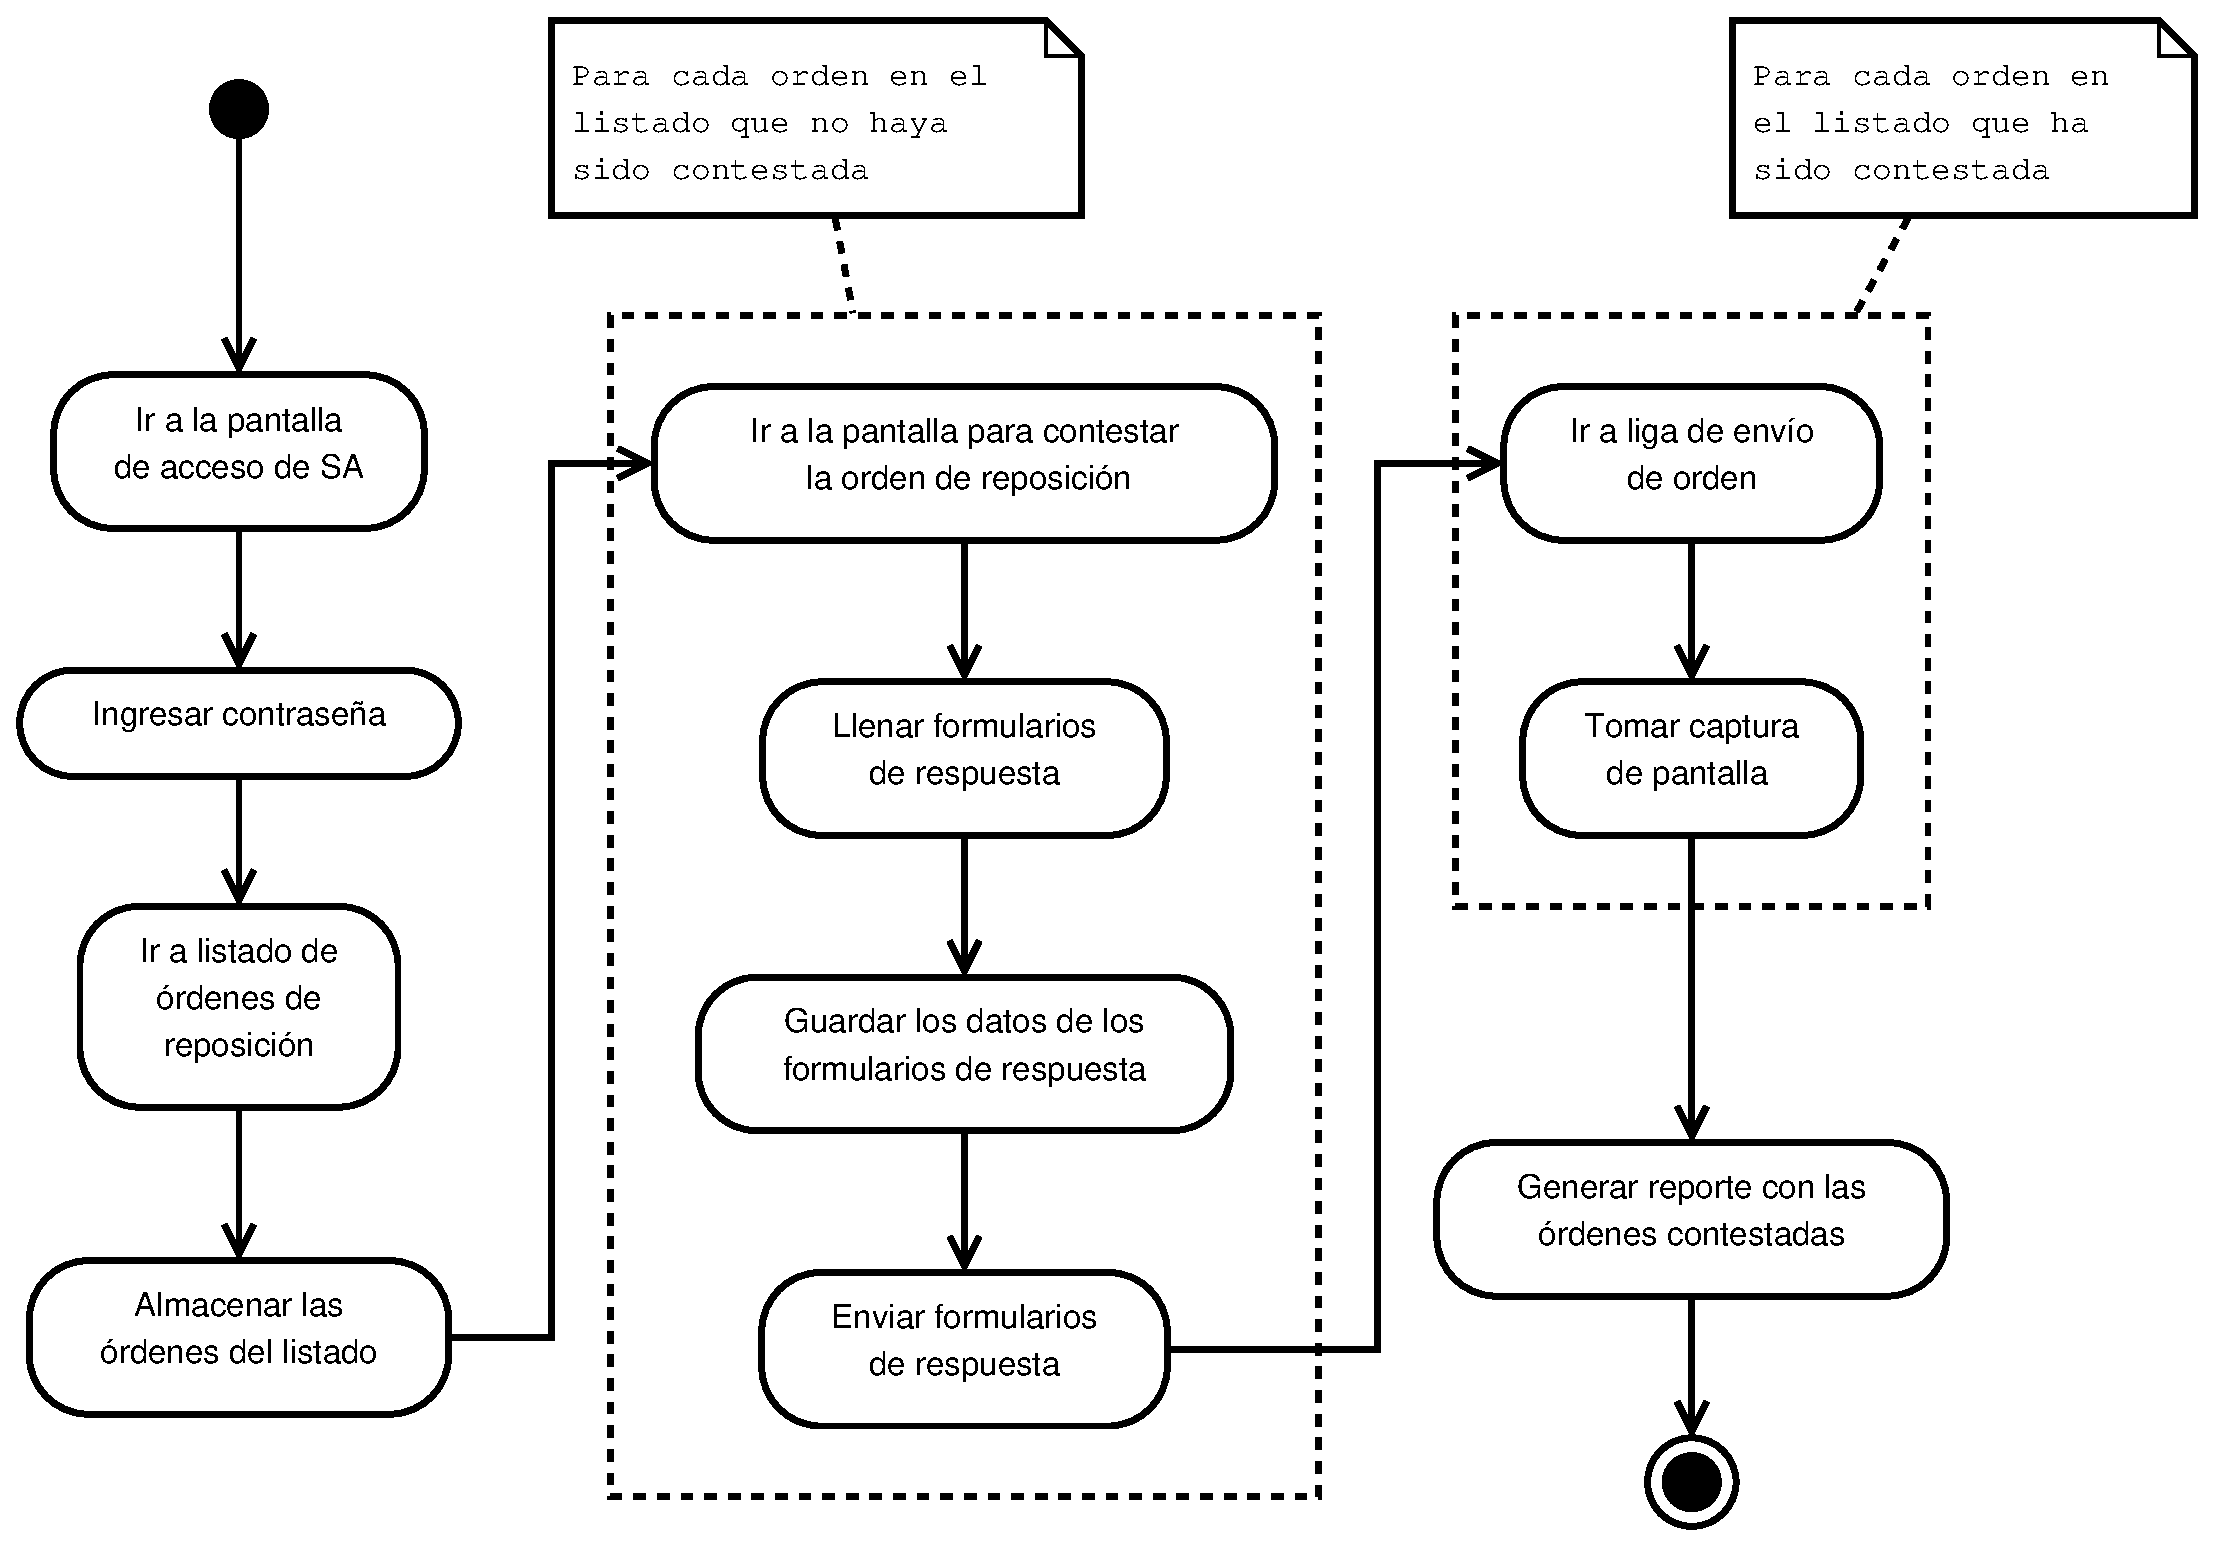
\includegraphics[scale=0.2]{dia-activity-contestar}
	\end{frame}
	\begin{frame}{Listado de órdenes de reposición}
		\begin{figure}[H]
		\centering
		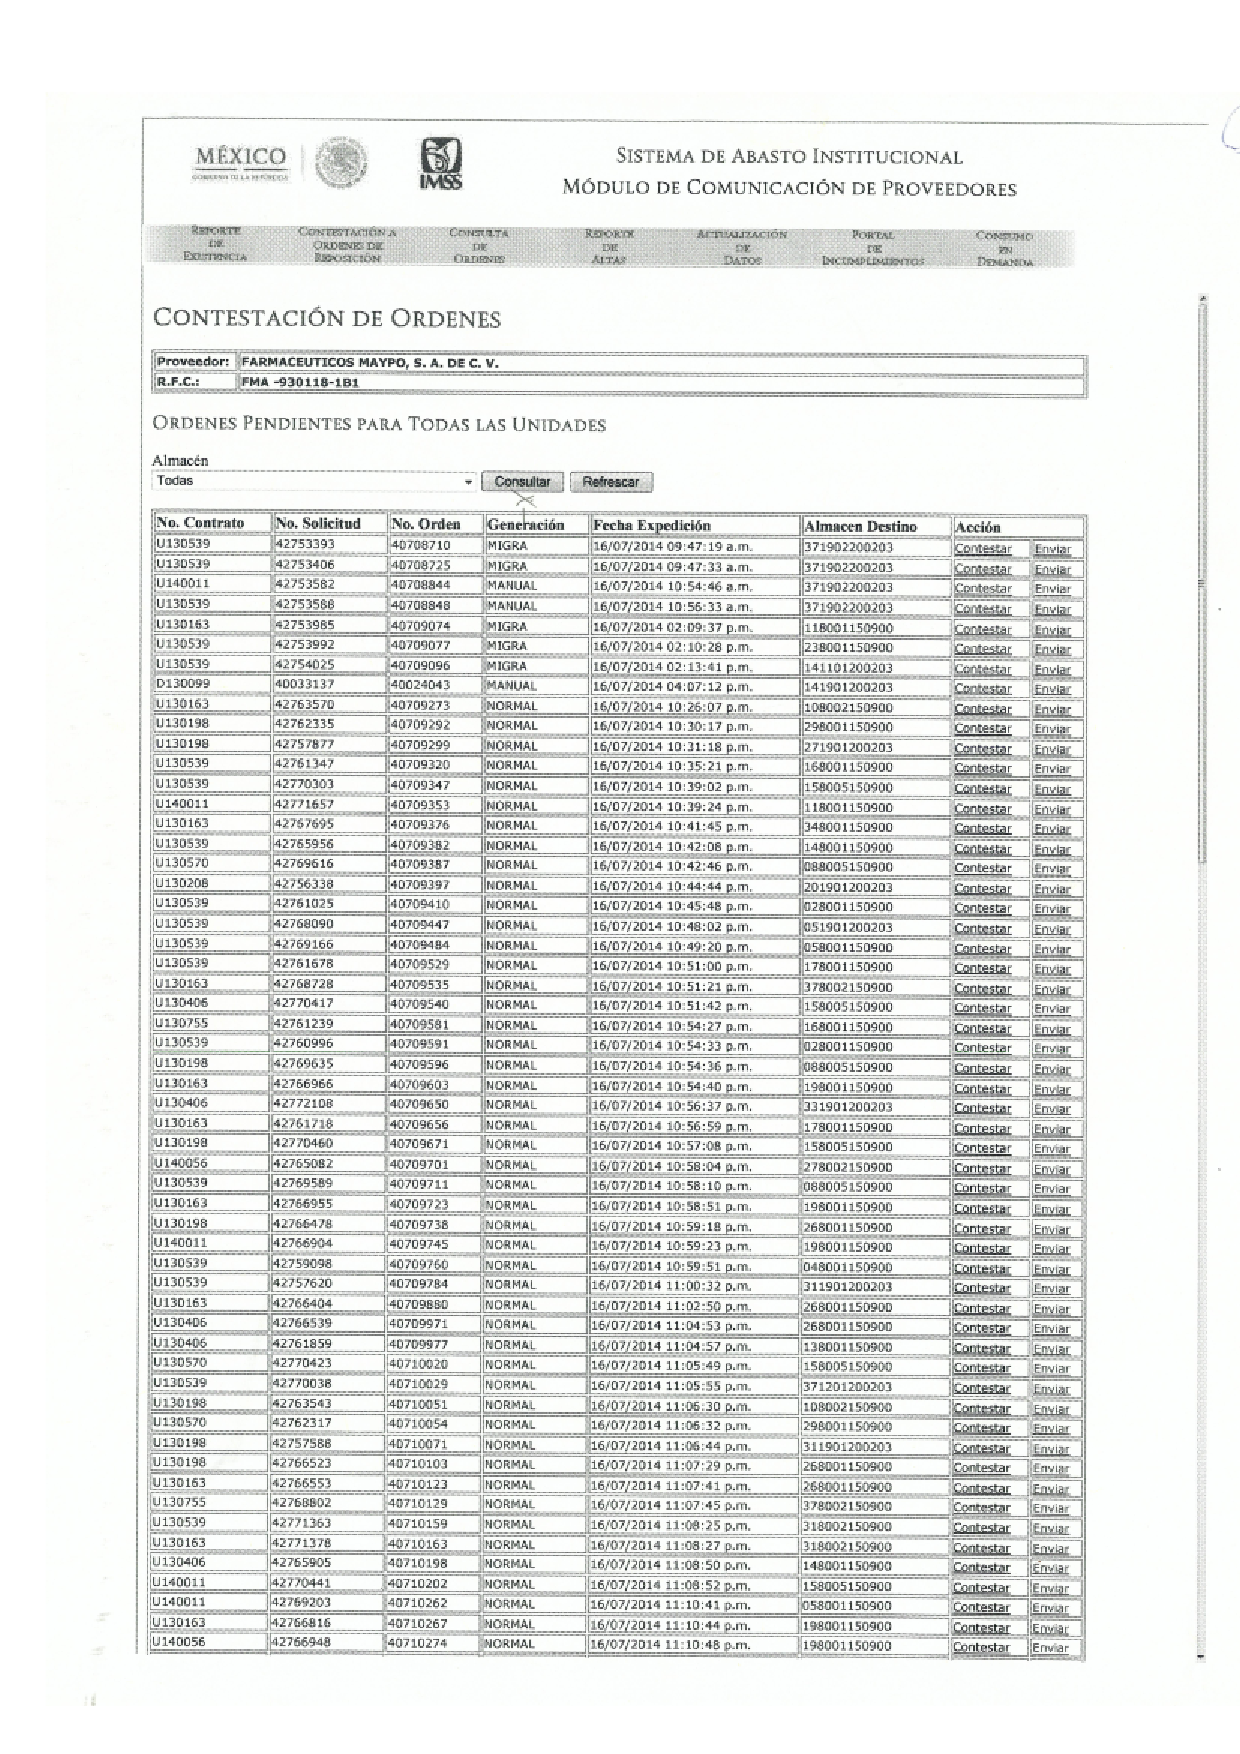
\includegraphics[width=\textwidth]{sai1}
		\label{fig:sai1}
		\end{figure}
	\end{frame}
	\begin{frame}{Respuesta a una orden de reposición}
		\begin{figure}[H]
		\centering
		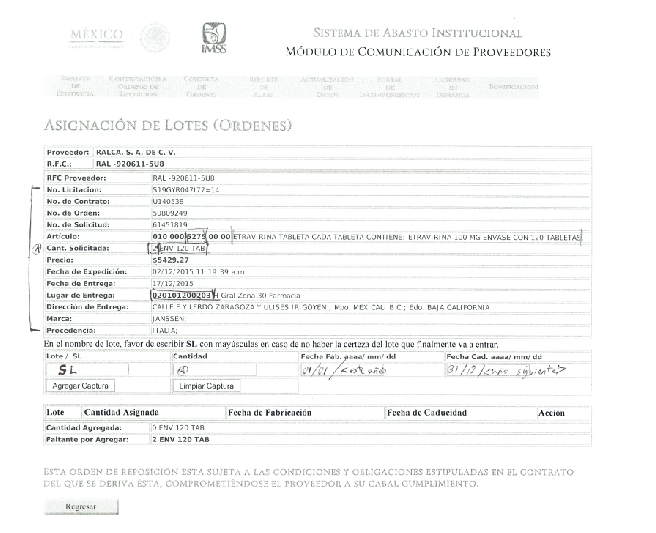
\includegraphics[scale=0.8]{sai2}
		\label{fig:sai2}
		\end{figure}
	\end{frame}
	\begin{frame}{Envío de una orden de reposición}
		\begin{figure}[H]
		\centering
		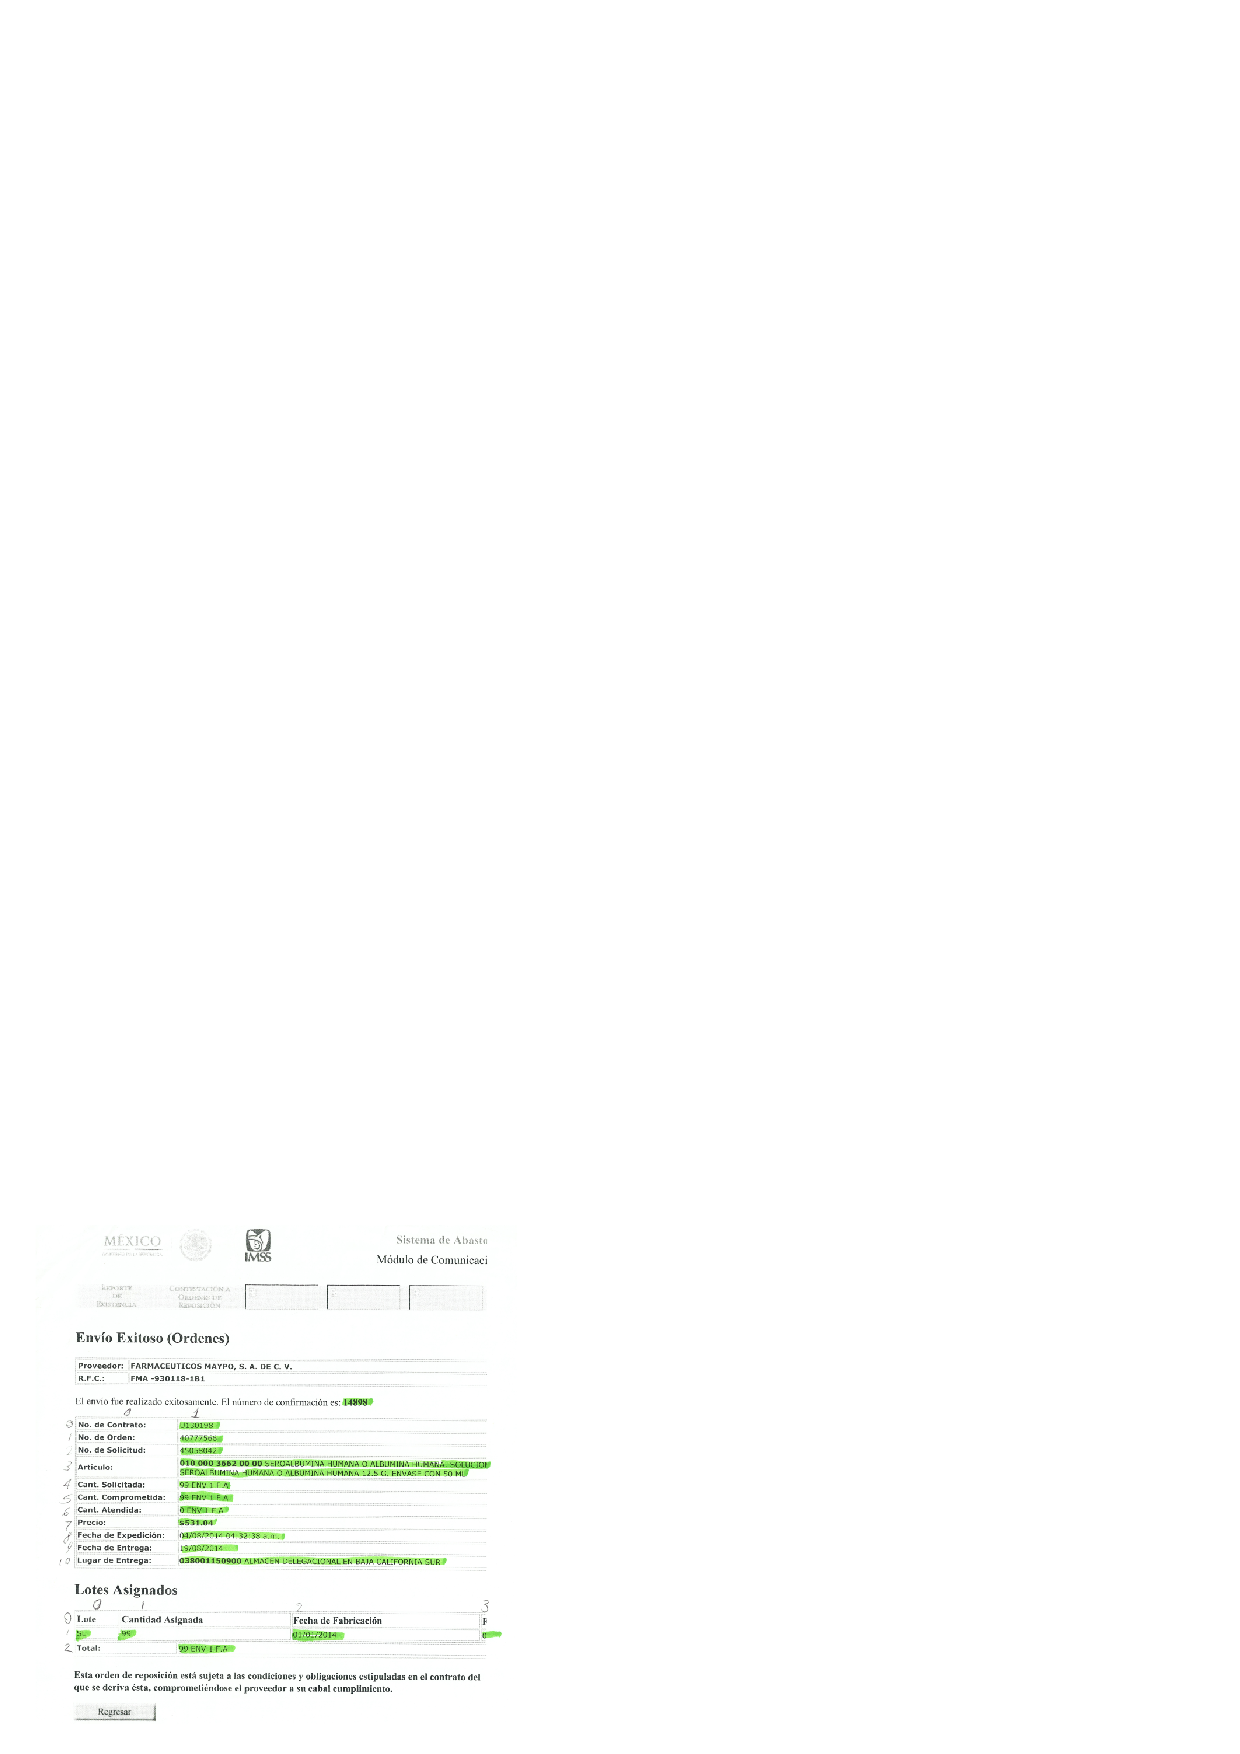
\includegraphics[scale=0.9]{sai4}
		\label{fig:sai4}
		\end{figure}
	\end{frame}
	\begin{frame}{Formato de salida}
		\begin{figure}[H]
		\centering
		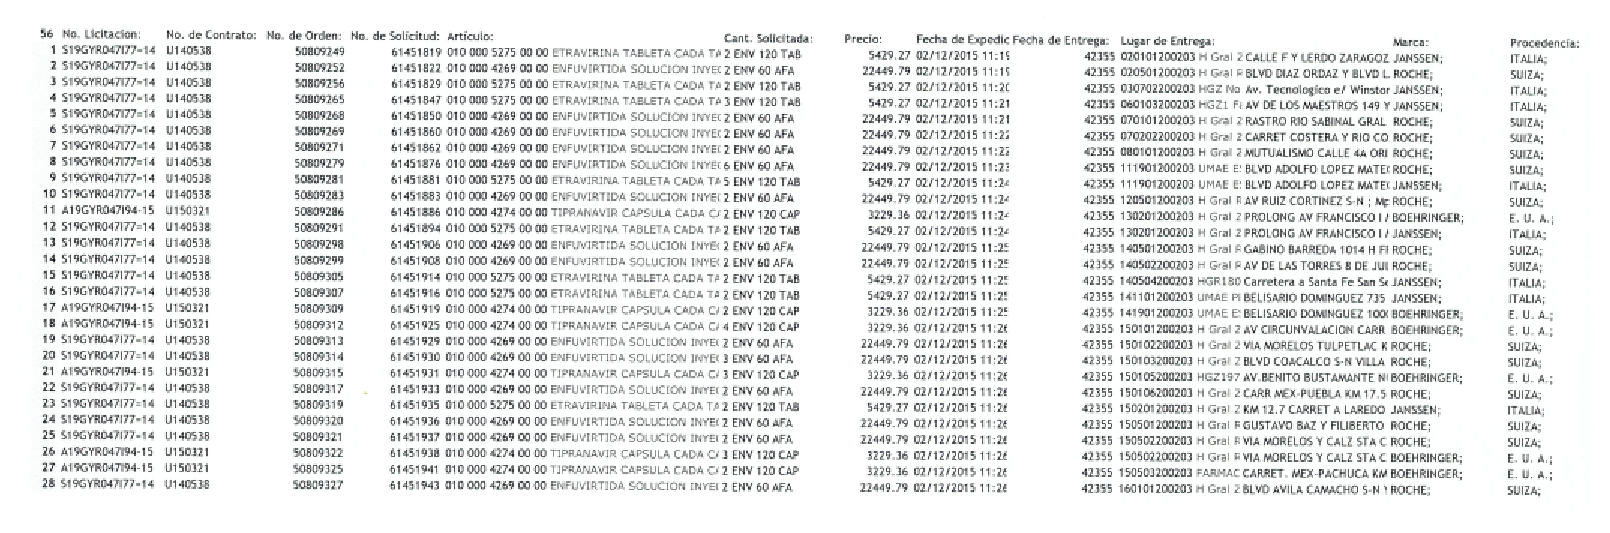
\includegraphics[width=\textwidth]{sai5}
		\label{fig:sai5}
		\end{figure}
	\end{frame}
	\begin{frame}{Diagrama de estados de las órdenes}
		\centering
		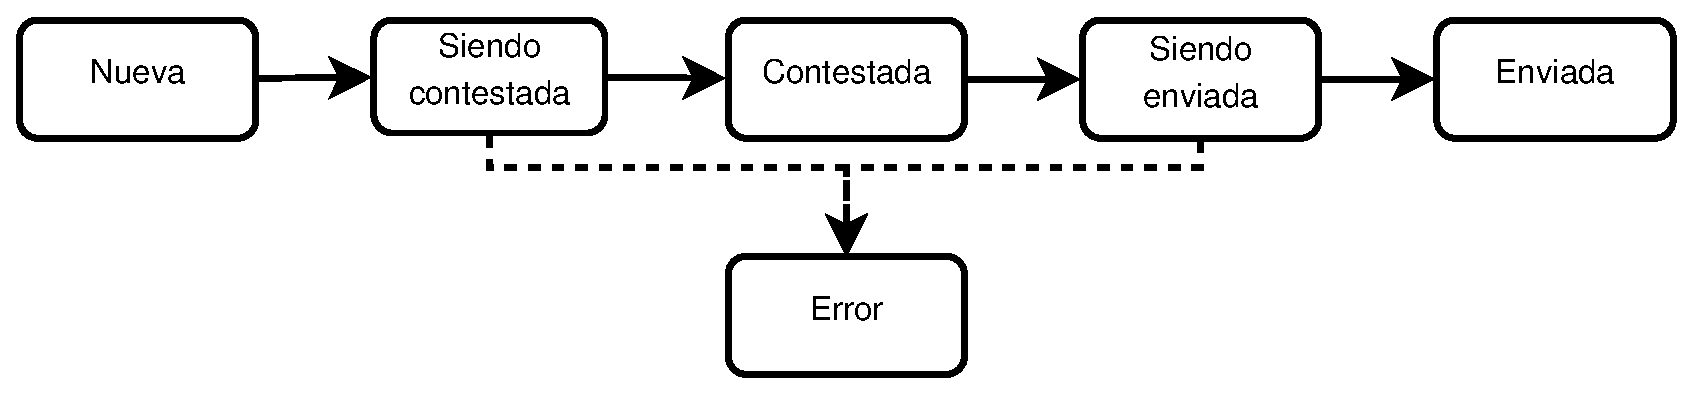
\includegraphics[width=\textwidth]{dia-estados-orden} 
	\end{frame}
	\begin{frame}{Automatización de la verificación}
		\centering
		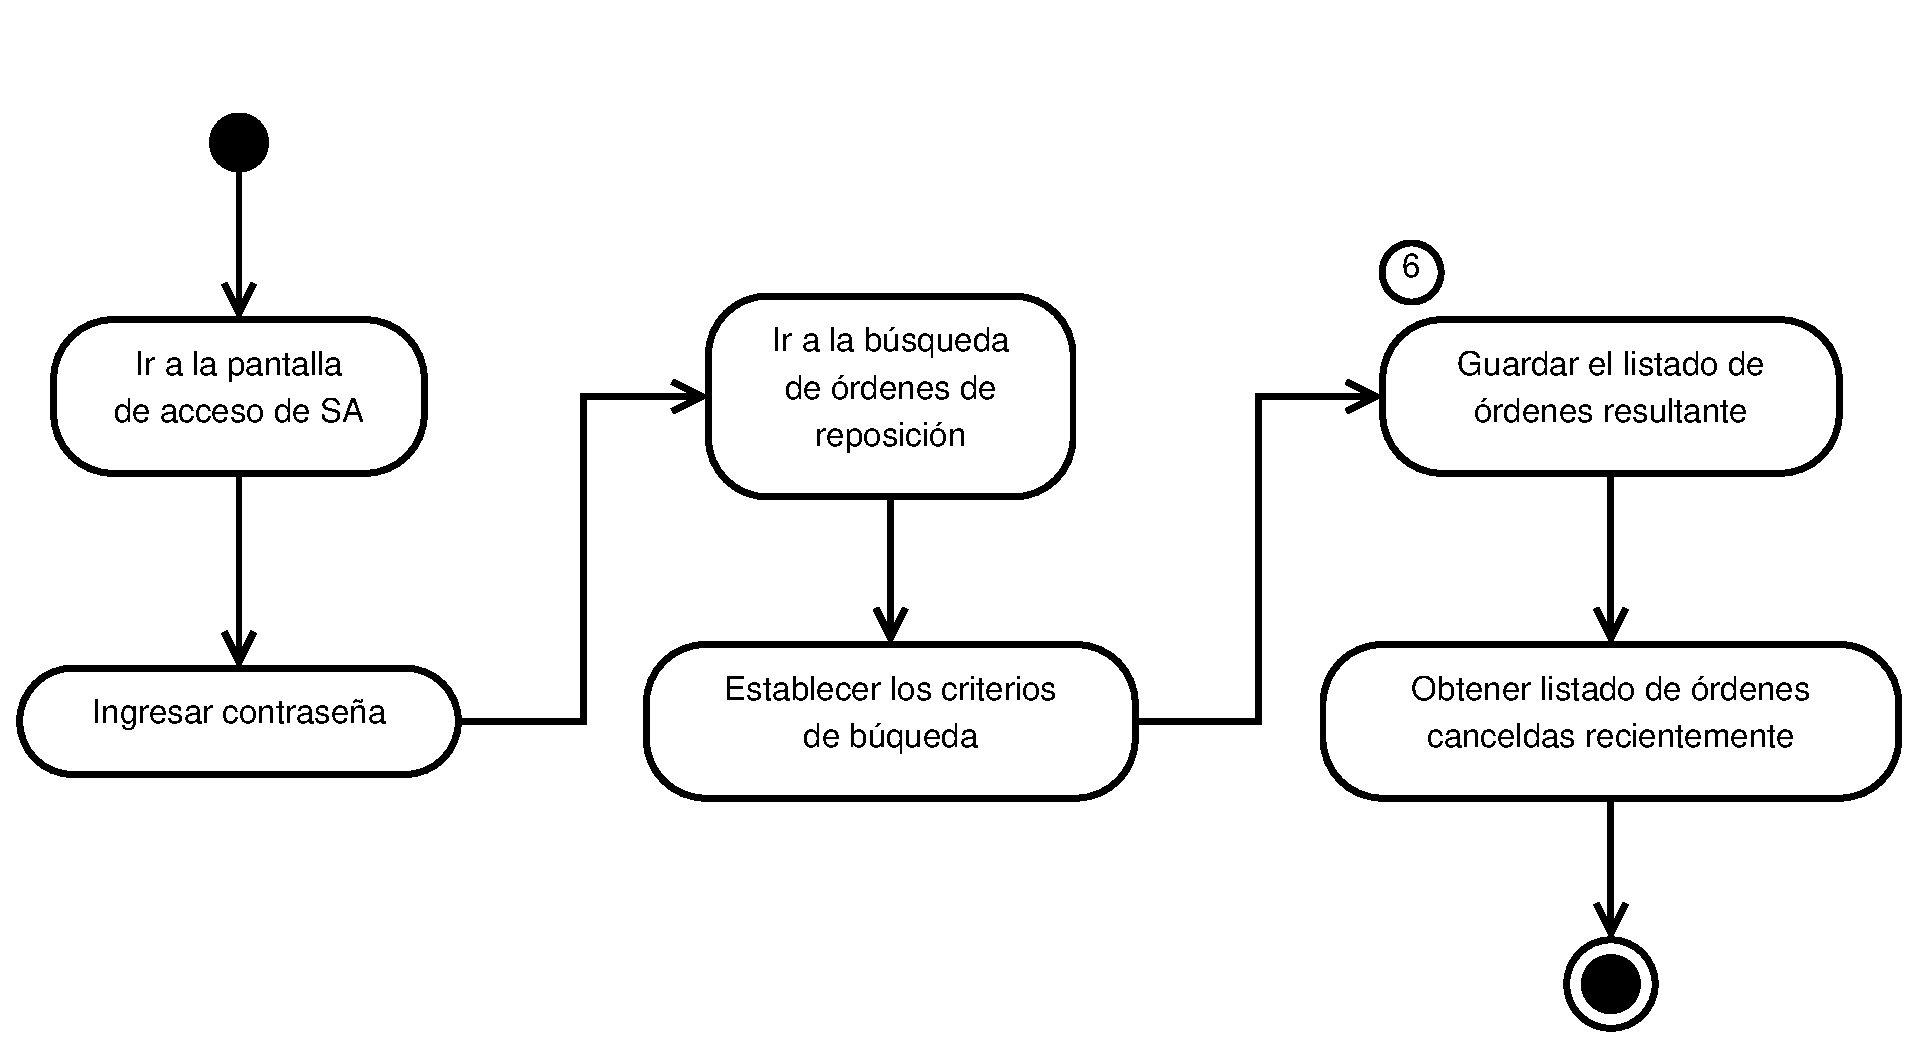
\includegraphics[width=\textwidth]{dia-activity-verificar}
	\end{frame}
	\begin{frame}{Navegación en la interfaz web}
		\centering
		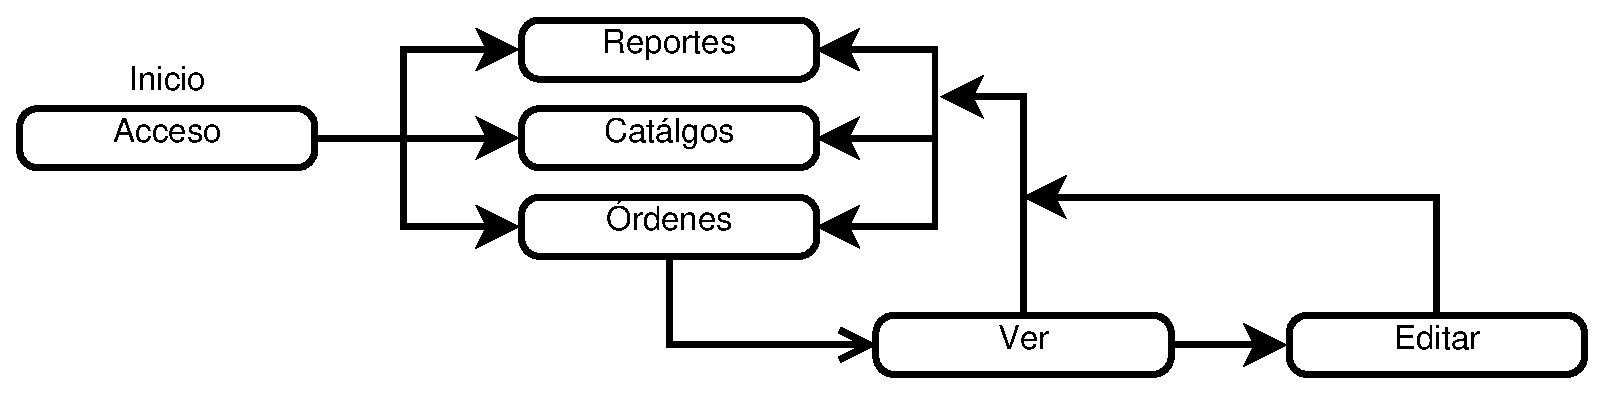
\includegraphics[scale=0.4]{dia-nav-flow}
	\end{frame}
	\begin{frame}{Acceso a la interfaz web}
		\centering
		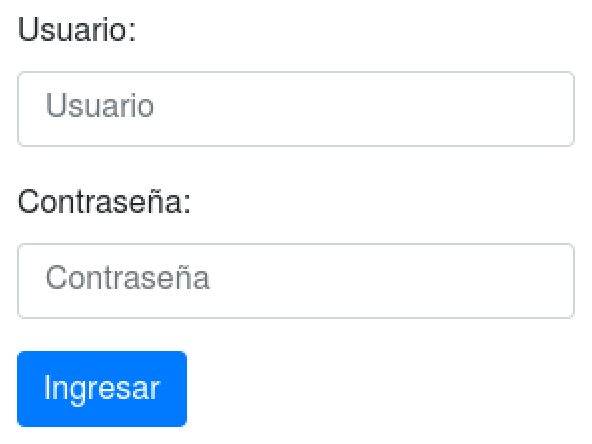
\includegraphics[scale=0.5]{maq-login} 
	\end{frame}
	\begin{frame}{Búsqueda de órdenes}
		\centering
		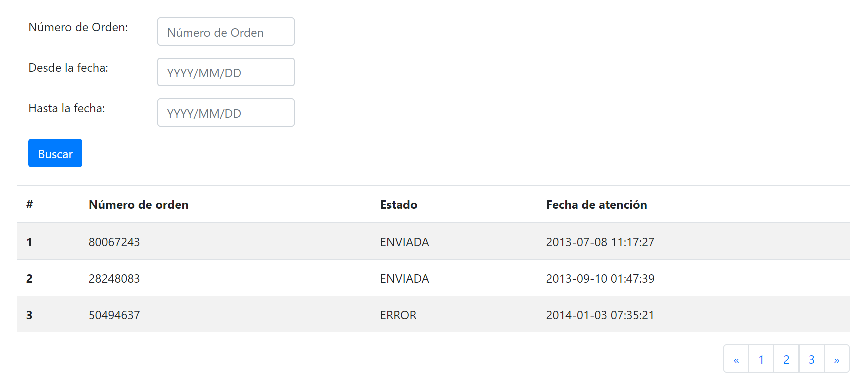
\includegraphics[width=\textwidth]{maq-search} 
	\end{frame}
	\begin{frame}{Visualización/Edición}
		\centering
		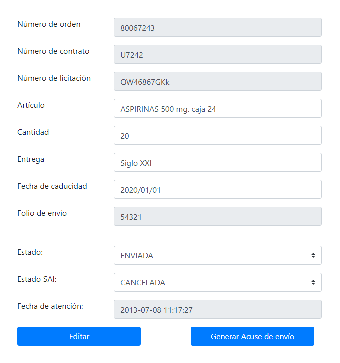
\includegraphics[scale=1]{maq-crud} 
	\end{frame}
	\begin{frame}{Generación de reportes}
		\centering
		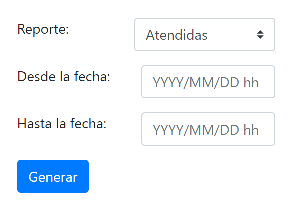
\includegraphics[scale=1.2]{maq-report} 
	\end{frame}
	\begin{frame}{Actualización de catálogos}
		\centering
		
\includegraphics[scale=1.3]{maq-upload}
	\end{frame}

\subsection{Requerimientos no funcionales}
	\begin{frame}{Requerimientos no funcionales}
		\begin{enumerate}
			\item Ejecución en sistema operativo Windows\textsuperscript{\textcopyright} o Unix.
			\item Base de datos relacional SQL.
			\item Uso de la herramienta \textit{Sahi}.
			\item Cifrado de contraseñar.
		\end{enumerate}
	\end{frame}

\subsection{Casos de uso}
	\begin{frame}{Casos de uso}
		\centering
		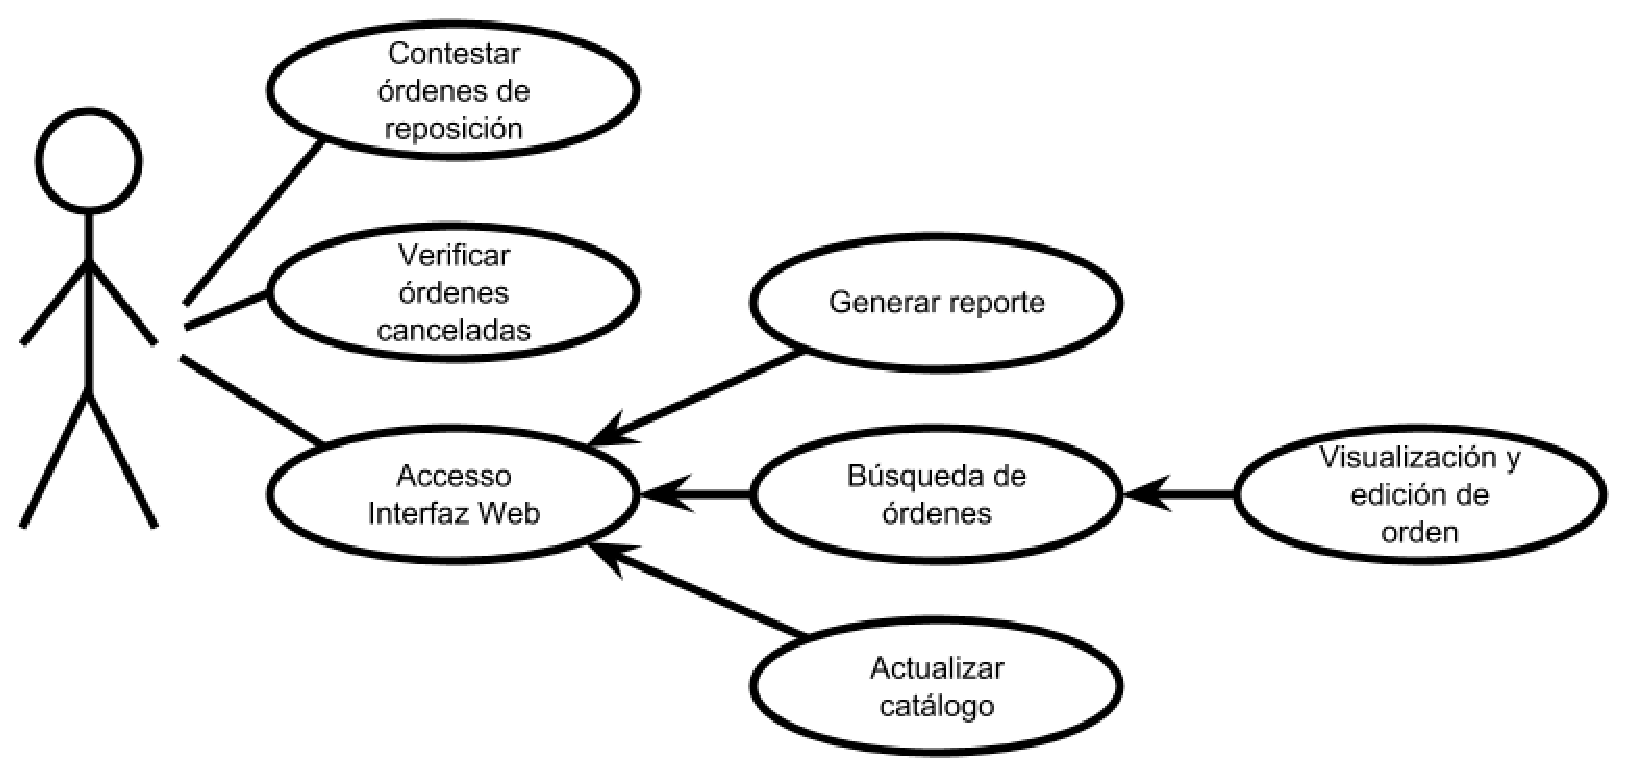
\includegraphics[scale=0.35]{dia-casos-uso} 
	\end{frame}

